%!TEX root = ../master_thesis.tex
\chapter{Background}
\label{ch:background}
In this thesis we work with methods from signal processing and machine learning. In this chapter, we first start with a gentle introduction to audio signal processing in Section~\ref{sec:asp} and build the premise for the later part of the thesis. Later we follow our discussion and build concepts of deep learning with particular focus on deep generative models in Section~\ref{sec:dgm}.

\section{Audio Signal Processing}
\label{sec:asp}
Audio signal processing (ASP) deals with the perception of sound to human auditory system. The physical form of sound or an audio can be seen as an encoding of air pressure over time. Formally, an audio signal is a function $x:\mathcal{R}\rightarrow \mathcal{R}$, that maps every point $t\in \mathcal{R}$ in time to sound pressure value $x(t)\in \mathcal{R}$. Such a representation is called analog or continuous time (CT) signal. When dealing with digital systems a critical step called digitization is used to process and store audio signals. Digitization is a two step process. The first step involves descritization of domain of a signal called as sampling. The second step involves approximation of range of a signal called as quantization. 

\textbf{Sampling} is a procedure to transform CT-signal to DT-signal. One common way to implement it is known as equidistant sampling. In an equidistant sampling, for a given CT signal $x:\mathcal{R}\rightarrow\mathcal{R}$ and a sampling constant $T>0$, a discrete time (DT) signal $x:\mathcal{Z}\rightarrow\mathcal{R}$ is derived as: 
\begin{equation}
\label{eq:sam}
x[n] = f(n.T)    
\end{equation}
for all $n\in \mathcal{Z}$. In this sampling scheme any two neighboring points are separated by a equal distance of $T$. The sampling rate of a signal is defined as number of samples per second given by $F_s=1/T$ and is measured in Hertz (Hz). Sampling in general is a non-invertible transformation and results in loss of information. However, for a band limited signal with a maximum frequency of $f_m$ sampling is invertible under Nyquist criterion that is $F_s\geq f_m$. The condition is known as \textbf{Nyquist Sampling Theorem}.


\textbf{Quantization} is a step to descritize real amplitude values using finite set of integer values. The general process involves the partitioning of the amplitude range in disjoint sets and using codebook to chose appropriate code value. A signal after digitization is an integer valued function $F:\mathcal{Z}\rightarrow\mathcal{Z}$. 

\subsection{Speech Processing}
The speech processing is the application of ASP to the understanding and analysis of speech signals. 
%The production of speech signals involves three main steps:  conceptualization, formulation, and articulation
\cite{meringer1999versprechen} describe speech signal as a composition of sequence of sounds produced by acoustical excitation of vocal tract. The vocal tract vibrates at a particular frequency which is called as fundamental frequency of the sound. The fundamental frequency of male speakers is generally in the range 50-200 Hz, of female speakers in the range 150-300 Hz and of children speakers in the range 200-400 Hz.  Figure~\ref{fig:speech_ex} part (a) gives an example of a speech signal of $10$ sec. sampled at $16$kHz. 

The speech signal are also referred as a slow time varying signal i.e. in a very short duration of time in 30-60 ms the characteristics of speech signals are stationary. To understand the acoustic properties of speech a common step involves decomposing it into fundamental components known as frequencies. 

In this thesis, we work with spectrogram representation of speech signals. In the following section, we will discuss the Fourier transform (FT) and other methods for time frequency representation. Since in this work we work with DT signals we will limit our discussion to the discrete case of FT.

%Based on the role of vocal tract in the production of speech the signals are divided into two categories: (i) Voiced  Speech (ii) Unvoiced speech
\subsection{Time Frequency Representation}
\label{subsec:timefreq_rep}
The Fourier transform (FT) is the widely used method of understanding time frequency dynamics of a signal. It maps a time domain signal to a frequency domain which provides an insight to the spectrum of frequency components composing the signal. In the book, The World According to Wavelets,~\cite{hubbard1998world} give a following elegant characterization of FT:

\emph{The Fourier transform is the mathematical procedure that breaks up a function into the frequencies that
compose it, as a prism breaks up light into colors. It transforms a function $f$ that depends on time into a
new function, $\hat{f}$, which depends on frequency. This new function is called the Fourier transform of the
original function (or, when the original function is periodic, its Fourier series).}

Formally, the Fourier transform (FT) of a DT signal $x\in \mathcal{R}^{L}$ is defined as:
\begin{equation}
    \hat{x}(k) = \sum_{n=0}^{L-1}  x(n).e^{-2\pi nkj/L}
\end{equation}

where $L$ is the length of signal, $k\in\{0,...,L-1\}$ and $e^{-2\pi nkj/L}$ are the complex frequency components in $x(k)$.
Each entry $\hat{x}(k)$ contains information about magnitude as well as phase of complex frequency component $e^{-2\pi nkj/L}$. Fourier transform is an invertible transformation and we can obtain time domain signal back from the frequency domain by summing the frequency component. Formally, an inverse FT of a signal $x\in \mathcal{C}^{L}$ is defined as:
\begin{equation}
    x(n) = \sum_{n=0}^{L-1}  \hat{x}(k).e^{2\pi nkj/L}
\end{equation}

The FT provides information about the frequency component of a whole signal. However, it fails to provide information about the temporal onset of frequencies thus is not helpful in the localization of frequencies i.e. in analyzing which frequency are present at any given point of time. In terms of speech signal, FT gives information about average sound events present in a signal but provides no information about which sound event occurred at a given time. Figure~\ref{fig:speech_ex} gives an example of FT of a speech signal. We can see it gives the overall measure of frequency but provides no information about the time location. To understand the nature and onset of frequencies we need a transformation which not only provides the spectral components but also provides the temporal properties of such components. To address this problem of time frequency localization, ~\cite{gabor1946theory} proposed a modified version of FT commonly referred as short time Fourier transform (STFT).

\begin{figure}
    \centering
    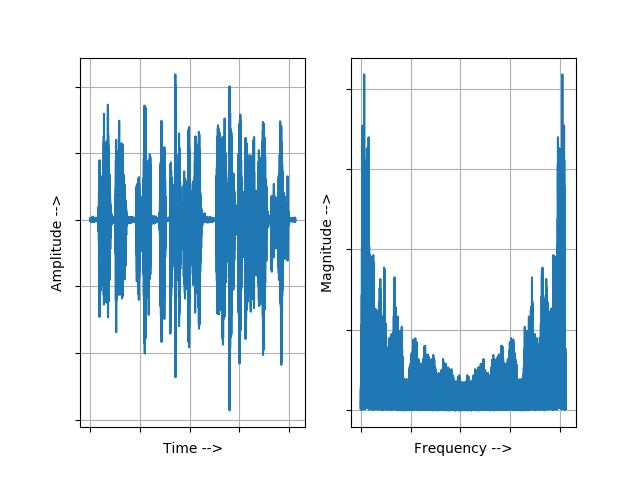
\includegraphics[width=0.75\columnwidth, height=0.40\columnwidth]{master_thesis_template/figs/fft.png}
    \caption{An example of time domain signal and its Fourier transformation.}
    \label{fig:speech_ex}
\end{figure}

\subsubsection{Short Time Fourier Transform}
The STFT or a time frequency representation of a signal can be thought of as a compromise between a time and a frequency representation. It provides a way to simultaneously represent time as well as frequency component of a signal thereby providing a way locate frequency events over time. The key idea behind STFT is to apply the FT locally over a signal using a window function. The window function is defined over an interval and provides a way to analyze frequency content of a signal in a given segment.

Formally, STFT of a signal $x\in\mathcal{R}^L$ with the window $w\in\mathcal{R}^L$, hop length $h\in\mathcal{N}$ and frequency steps $M\in\mathcal{N}$  is defined as:
\begin{equation}
    \hat{X}_w(a,b) = \sum_{l=0}^{L-1} x(l).w(l-nh)e^{-2\pi jab/M}
\end{equation}
for all $a\in\{0,...,N-1\}$ and $b\in\{0,...,M-1\}$. The hop length $h$ is a measure of redundancy it is defined as number of time steps between two consecutive window frames. Depending on sampling frequency and hop length we can also express frequency step $a$ in Hz as $\Tilde{a} = a.F_s/N$ and time step $b$ in seconds as $\Tilde{b}=b.h/F_s$, where $F_s$ is the sampling rate of signal $x$. The entry $X(a,b)$ represents Fourier coefficient present at the $a^{th}$ frequency and $b^{th}$ time step. 

Similar to FT we can also define inverse transformation for STFT. For a given STFT matrix $\hat{X}_w$ under $\hat{w}$ an inverse STFT is defined as:
\begin{equation}
    x(n) = \sum_{a=0}^{N-1} \sum_{b=0}^{M-1} \hat{X}_w(a,b).\hat{w}(n-ha)e^{2\pi jab/M}
\end{equation}

where $\hat{w}$ is a FT representation of window $w$. The window size controls the time frequency resolution, smaller window size in time domain gives good time resolution but bad frequency resolution. Likewise large window size gives better frequency resolution but bad time resolution. The simultaneous time frequency analysis is governed by Heisenberg Uncertainty principle. Improving resolution in one domain effects the quality in the other domain and viceversa. Fortunately, the Gaussian window have minimum uncertainity and are a preferred choice for STFT. In this work we use a type of Gaussian window called as Hanning window originally proposed in~\cite{harris1978use}. 

The STFT matrix has two parts: magnitude and phase information. Due to complexities in dealing with phase information discussed in later part in Section~\ref{subsec:phrecon}, magnitude information is a preferable representation for machine learning tasks. The magnitude of a STFT matrix $\hat{X}_w(a,b)$ is defined as $\mathopen|\hat{X}_w(a,b)\mathclose|$.
In Figure~\ref{fig:time_freq_rep} part (a) gives an example of STFT of a signal with Gaussian window. The coloured region in spectrogram reflect the magnitude of coefficients. A log transformation defined as: $\ln(1+\mathopen|\hat{X}_w(a,b)\mathclose|)$ is commonly applied on magnitude spectrogram to enhance the low magnitude coefficients. Figure~\ref{fig:time_freq_rep} part (b) gives an example of log transformation.


\subsubsection{Mel Spectrogram}
Human ears perceive the perceptual difference in sound quality based on the pitch of a signal. The pitch is a function of frequency and can be interpreted as the perceived frequency. The mel scale introduced by~\cite{stevens1940relation} is a transformation which relates the real frequency to the perceived frequency a.k.a pitch. Various forms of mel functions have been proposed one commonly used transformation is given by:
\begin{equation}
    m = 2595 \log(1+\frac{f}{700})
\end{equation}
mapping frequency $f$ in Hz to $m$ mels.
The magnitude spectrogram consists of different bands of frequency. To perceive harmonics of each band it is essential that all bands have equal resolution on mel scale. This is achieved by applying bank of overlapping triangular filters around center frequency of each band. The Mel spectrogram is obtained by scaling magnitude spectrogram to mel scale and then passing it through filterbanks. For further details on mel filterbanks we refer to~\cite{kopparapu2010choice}. Figure~\ref{fig:time_freq_rep} gives an example of mel spectrogram and its comparison with the magnitude and log magnitude representation.
%\begin{figure}
%    \centering
%    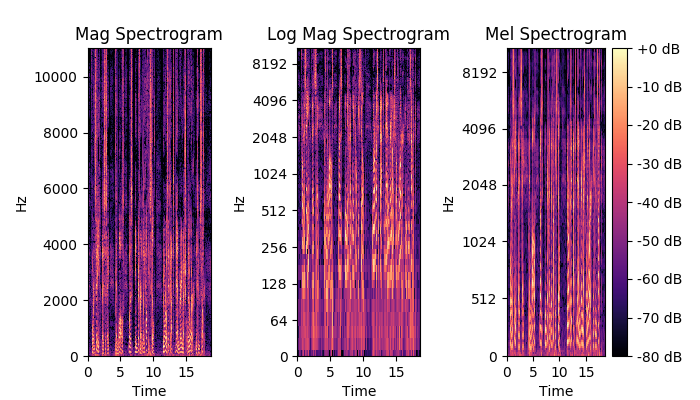
\includegraphics[width=0.95\columnwidth, height=0.40\columnwidth]{master_thesis_template/figs/freq_res.png}
%    \caption{Time frequency representation of signal illustrated in Figure~\ref{fig:speech_ex}. On left is the magnitude spectrogram, in middle is the log magnitude spectrogram and on right is the mel spectrogram. For this example we use $1024$ point fft with $75\%$ overlap, hanning window of size $1024$ and $128$ mel filters.}
%    \label{fig:time_freq_rep}
%\end{figure}

\subsection{Phase Reconstruction}
\label{subsec:phrecon}
The STFT representation $\hat{X}$ is a matrix of complex numbers. The squared-magnitude of this matrix is interpreted as an energy spectra where each entry $(a,b)$ represents the energy of signal at the frequency step $a$ and time step $b$.
However, such interpretation is not clear for phase spectra of STFT matrix $\hat{X}$. This increases the complexity of analysis. As a consequence, magnitude information of STFT matrix is a preferable choice for various signal processing and machine learning task.

\begin{figure}
    \centering
    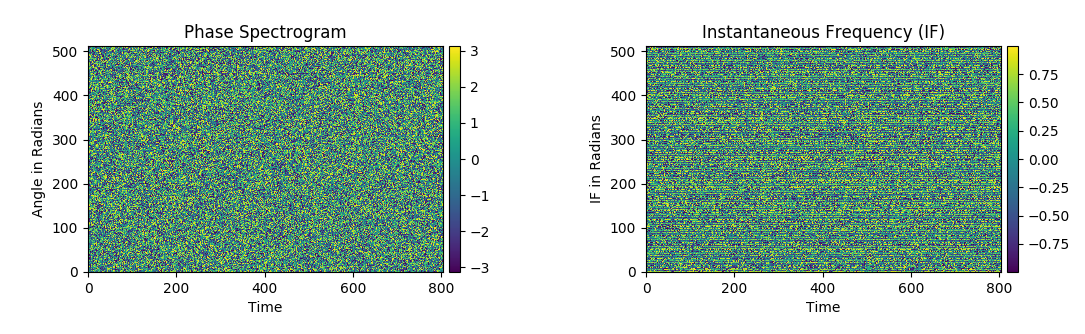
\includegraphics[width=0.75\columnwidth, height=0.40\columnwidth]{master_thesis_template/figs/phase_res.png}
    \caption{On left is time phase representation of signal and on right is the instantaneous frequency (IF) representation of a signal illustrated in Figure~\ref{fig:speech_ex}.}
    \label{fig:phase_response}
\end{figure}

One problem with this choice is the consistency of spectrogram under any transformation. The windowing in STFT is done with overlapping time frames. To preserve time-frequency dynamics any transformation on STFT should take also into account this information. However, signal processing as well as machine learning transformations on magnitude spectrogram often ignore this information. As a result the modified magnitude spectrogram might not even have any valid time domain reconstruction. Thus to reconstruct a signal a crucial requirement is an appropriate phase information which in turn is guaranteed if the spectrogram representation is consistent.

%However, for application like speech synthesis magnitude information is not sufficient to infer time domain signal.
\subsubsection{Spectrogram Consistency}
As discussed previously any transformation applied on magnitude spectrogram representation makes it difficult to reconstruct the time domain signal. In this work we generate spectrogram using GAN, we discuss it in detail in later part of the thesis~\ref{ch:unvc}. One central problem underlying generation is the consistency of spectrogram that is to say finding a unique time domain signal from a generated  spectrogram representation. In this part we formally define the condition for consistency of spectrogram.

Let $\mathcal{C}^{M N}$ be a space of complex matrices, $\mathcal{H}^L$ be a space of time domain signals and $\mathcal{V}^{M N}$ be a space of consistent spectrogram. A consistent spectrogram $X\in\mathcal{V}^{MN}$  for some $x\in\mathcal{H}^L$ is a matrix which can be obtained by STFT of $x$. Since, $\mathcal{V}^{MN} \subset \mathcal{C}^{MN}$ $\exists  $W$\in\mathcal{C}^{MN}$ s.t. there is no unique reconstruction of $W$ in $\mathcal{H}^L$. Thus for any $W\in\mathcal{C}^{MN}$ to be a consistent spectrogram it should be in a null space of a linear transformation $\mathcal{F}$ defined as:
\begin{equation}
\label{eq:null}
    \mathcal{F}(W) = \text{STFT}(\text{ISTFT}(W)) - W
\end{equation}


\begin{figure}
    \centering
    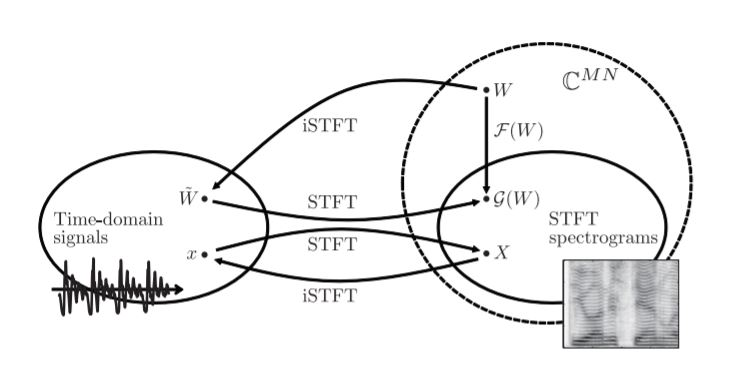
\includegraphics[width=0.55\columnwidth]{master_thesis_template/figs/spec_consistency.JPG}
    \caption{An example of spectrogram consistency. Taken from~\cite{le2010fast}}
    \label{fig:spec_con}
\end{figure}
\subsubsection{Griffin Lim Reconstruction}
Griffin Lim Algorithm (GLA) proposed by~\cite{griffin1984signal} uses consistency constraint to reconstruct closest time domain signal from a modified magnitude spectrogram. The GLA finds phase for a magnitude spectrogram by projecting it into null space of operator $\mathcal{F}(W)$. Thus it minimizes the projection error in Eqaution~\ref{eq:null} by iteratively projecting signal across two domain i.e. from frequency to time and time to frequency. Under sufficient overlap in STFT spectrogram, GLA guarantees to reconstruct a unique solution approximating the signal. Algorithm~\ref{alg:gla} further defines the GLA.
\begin{algorithm}
\caption{Griffin-Lim Algorithm}
\label{alg:gla}
\begin{algorithmic}[1]
\Procedure{GLA}{$\mathcal{\hat{M}},\mathcal{N}_{iter}$} \Comment{Input: Modified Magnitude Spectrogram and number of training iterations}
\State $\phi_0$ $\leftarrow$ $\angle$ $\mathcal{N}(0,I)$ \Comment{Initial random phase in radians}
\State $\hat{\mathcal{S}}_o = \mathcal{\hat{M}}.e^{-j\phi_o}$ \Comment{initial full spectrogram}
\For{i \text{in} \textbf{range (}1, $\mathcal{N}_{iter}$\textbf{)}} 
\State $\hat{\mathcal{S}}_i$ = $\text{STFT}$\{$\text{ISTFT}\{\hat{\mathcal{S}}_{i-1}$\}\}
\EndFor
\State x = $\text{ISTFT}$\{$\hat{\mathcal{S}_n}$\}
\State \textbf{return} x
\EndProcedure
\end{algorithmic}
\end{algorithm}

One problem often encountered with GLA is low quality reconstruction when dealing with high quality sound signals. Many improvements of the GLA have been proposed.~\cite{perraudin2013fast} formulate phase reconstruction as an optimization problem and modify conventional GLA.~\cite{pruuvsa2017noniterative} utilized phase magnitude relationship proposed by~\cite{auger2012phase} and proposed a stable way to integrate magnitude spectrogram at different scale. In this work we limit our discussion to GLA. For further details we refer to~\cite{perraudin2013fast},~\cite{le2010fast},~\cite{jaganathan2015phase}.
\section{Deep Generative Models}
\label{sec:dgm}
In this section, we build our discussion around deep generative models. We will start with a gentle introduction to deep learning in Section~\ref{subsec:dl}. We will then discuss about generative models in Section~\ref{subsec:gm} and will finally conclude our discussion with generative family of models based on neural networks in Section~\ref{subsec:gan},~\ref{subsec:vae} and~\ref{subsec:cgan}. 
\subsection{A short introduction to Deep Learning}
\label{subsec:dl}
In recent years deep learning (DL) has emerged as a popular choice for modeling various artificial intelligence (AI) tasks ranging from object recognition in computer vision to language models in NLP. DL works on the principle of building solution to a complex problem by decomposing it into simpler ones which reduces the complexity of problem and provides insights to model non-linear dynamics of data. 

~\cite{Goodfellow-et-al-2016} outline DL as:
\emph{A way to allow computers to learn from experience and understand the world in terms of a hierarchy of concepts, with each concept defined through its relation to simpler concepts. By gathering knowledge from experience, this approach avoids the need for human operators to formally specify all the knowledge that the computer needs. The hierarchy of concepts enables the computer to learn complicated concepts by building them out of simpler ones. If we draw a graph showing how these concept defined as the decomposition of complex concepts into simple ones and the recombination into new complex concepts. An algorithm therefore has to establish a hierarchy of concepts. A visualization of this hierarchy would be a multi-layered graph, that can be called deep in a graph theory context.}

\subsubsection{Artificial Neural Network}
\label{sub:ann}
Artificial Neural Network (ANN) is a learning model inspired by working of biological neurons. It consists of an arbitrary number of small computational units called artificial neurons and solves learning problem by modeling the strength of connection between them. This nature of ANN allows them to model functions of arbitrary complexity and thus classifies them as the universal approximators~\cite{hornik1989multilayer}.

We start our discussion with the basic form of ANN commonly referred as \emph{perceptron}. The \emph{perceptron} use single neuron to approximate the function. Following~\cite{mitchell1990machine} we define the perceptron model as follows: for an input $x\in\mathcal{R^D}$ and the parameterized function $f:x\rightarrow y$ defined as $f(x;w,b)=w^Tx+b$ where  $y\in\mathcal{R}$ is an output score, $w\in\mathcal{R^D}$ is a weight parameter and $b\in\mathcal{R}$ is a bias term. For a binary classification task the output $f(x;w,b)$ is further passed through the decision function also referred as
\emph{activation function} formally given by Equation~\ref{eq:act_fun}. 
\begin{equation}
\label{eq:act_fun}
  \hat{y}= 
\begin{cases}
    1,& \text{if } f(x;w,b)> 0\\
    0,              & \text{otherwise}
\end{cases}  
\end{equation}

The initial parameters $(w,b)$ are set to zeros. At every step of learning the output $y$ is computed and the parameters are adjusted based on the mean-squared-error between target and predicted output. One major limitation of \emph{perceptron} is it cannot model non-linear relations. For instance, \texttt{XOR} function. 

\emph{Multilayer perceptron} (MLP) is a class of ANNs which unlike perceptron uses multiple neurons over several layers to approximate the unknown function. The interconnected neurons form a hierarchical network which allows to model function of arbitrary complexity. In addition, there are various families of activation function which further benefit the learning process.

Formally, MLP can be considered as a chain of functional maps applied on data to unravel the non-linearities over several layers of hierarchy. Let $L$ be number of layers, $x\in\mathcal{R}^d$ be an input representation, for a layer $l$: $d_l\in\mathcal{N}$ be number of neurons, $v^{l}$ be an input representation, $u^{l}$ be an output representation, $f_l:\mathcal{R}^{d_{l-1}}
\rightarrow\mathcal{R}^{d_{l}}$ be a transformation mapping $u^{l-1}$ to  $u^l$, let $\theta^{l-1,l}=\{w^{l-1,l},b^{l-1,l}\}$ be parameters connecting layer $l-1$ to $l$ and $\sigma^{l}$ be a activation function, then the output of MLP $f(x)$ is defined as:
\begin{equation}
\label{eq:mlp}
\begin{aligned}
    v^{0}(x) = x\\
    v^{l}(x) = u^{l-1}(x)\\
    u^{l}(x) = \sigma^l(f^{l}(v^{l},\theta^{l-1, l}))\\
    f^{l}(v^{l},\theta^{l-1, l}) = w^{l-1, l}.u^{l}+b^{l-1,l}\\
    f(x) = u^{L}\circ u^{L-1}\circ...\circ u^{1}\circ u^{0}(x)
\end{aligned}
\end{equation}

The MLPs are efficient in modeling any class of functions. However, it is difficult to train MLPs with large number of neurons in hidden layers. This is because each neuron connects to all the neurons of previous layer. As a result number of parameters increase significantly making learning infeasbile. The another issue with MLP is they are permutation invariant i.e. if the feature space is shuffled the output of network is still same. As a result it fails in modeling spatial relationship in data. For further details we recommend readers to refer to~\cite{Goodfellow-et-al-2016}.


\subsubsection{Convolutional neural network}
\label{sub:cnn}
Convolutional neural networks (CNN)~\cite{lecun1995convolutional} take the inspiration from the receptive field of the visual cortex. In visual cortex neurons form local regions called receptive field a.k.a feature map where neurons responds selectively to various attributes of a visual input. The CNN exploit this idea to  implement local feature maps which by weight sharing learns different level of abstractions from a given input.  

A convolution is a linear operator which takes two functions as an input and provides another function as an output. This composition is defined to capture the \emph{cross-correlation} between the two functions. Formally, for an input $x\in \mathcal{R}^N$ and a receptive field in $w\in \mathcal{R}^K$ the convolution operator is defined as:
\begin{equation}
\label{eq:conv}
    y(n) = (x * w)(n)  = \sum_{k=0}^{K} x(k).w(n-k)
\end{equation}
where $n\in\{0,...,N+K-1\}$. Likewise, convolution operator can be extended to multidimensional input $x\in\mathcal{R}^{M_1\times M_2\times ...M_d}$. For more comprehensive explanation we refer to~\cite{Goodfellow-et-al-2016}.

The CNN uses convolutional operator to apply parametric transformation on the input representation. Thus learning parameters which are effective in capturing spatial or temporal correlation in the data. For an input $x\in\mathcal{R}^{m\times n \times c}$, the convolutional layer  $l\in L$ with filter maps $w\in\mathcal{R}^{k_l \times k_l \times c_{l-1}}$ in CNNs is a three step operation: (i) Apply convolutional operator $f_l:\mathcal{R}^{m_{l-1}\times n_{l-1}\times c_{l-1}} \rightarrow\mathcal{R}^{m_{l}\times n_{l}\times c_{l}}$ to obtain intermediate output. (ii) Apply activation function $\sigma^{l}$ and (iii) Apply pooling operation $g_l^d:\mathcal{R}^{m_{l}\times n_{l}\times c_{l}}\rightarrow \mathcal{R}^{m_{l/d}\times n_{l/d}\times c_{l}}$ to downsample the output of activations, where $c_0 = c$ are input channels.

Depending on the design choice, the step (iii) can also be omitted sometime. An optimal choice of number of filter maps and its size is an hyperparameter optimization problem and is usually decided by heuristics or grid search. A stack of convolutional layers followed with some layers of MLP is a preferrable design choice of CNNs and have shown a lot of success particularly in computer vision tasks like object recognition~\cite{krizhevsky2012imagenet}, ~\cite{donahue2014decaf}. However, for tasks like super resolution or object localization where the output is essentially in spatial domain
a fully convolutional (FCN) approach is a preferred design choice. The FCN learn a path from pixels in the first layers to the pixel in the deeper layers thus preserving point to point correspondence and produce an output in the spatial domain. 

%In addition,  $W^{l}_{l-1}$ is defined for every receptive field $q\in Q$ as a local region $W^{l, q}_{l-1}\in\mathcal{R}^{k\times k\times c}$, where $k$ is the size of receptive field, $c$ is the number of channels in an input and $m\times n$ is the dimensionality of each input channel.

%For an input $x\in\mathcal{R}^{m\times n \times c}$, for a layer $l$: $V^{l}$ be an input representation, $U^{l}$ be an output representation, and filter maps $w\in\mathcal{R}^{k_l \times k_l \times c_{l-1}}$

%$f_l:\mathcal{R}^{d_{l-1}}\rightarrow\mathcal{R}^{d_{l}}$ be a transformation mapping $U^{l-1}$ to  $U^l$, $\theta^{l-1,l}=\{W^{l-1,l},b^{l-1,l}\}$ be parameters connecting layer $l-1$ to $l$ and $\sigma^{l}$ be a activation function


 %the convolution operator for arbitrary layer $l$ with $c_l$ kernels is defined as:
%\begin{equation}
%    \begin{aligned}
%    V^{0}_{c_0}(x) = x\\
%    V^{l}_{c_l}(x) = U^{l-1}_{c_l}(x)\\
%    U^{l}_{c_l}(x) = \sigma^l(f^{l}(V^{l}_{c_l},\theta^{l-1, l}_{c_l}))\\
%    f^{l}(V^{l}_{c_l},\theta^{l, l-1}_{c_l}) = W^{l-1, l}_{c_l}*_{c_l} U^{l}_{c_l}+b^{l-1,l}_{c_l}\\
%    f(x) = U^{L}_{c_L}\circ U^{L-1}_{c_{L-1}}... U^{1}_{c_1}\circ U^{0}_{c_0}(x)        
%    \end{aligned}
%\end{equation}


\subsubsection{Residual Networks}
\label{sub:resnet}
The training of deep neural networks is difficult. The increasing depth results in the saturation of the performance followed with a rapid degradation. The residual networks (ResNets) introduced by~\cite{he2016deep} address this problem by proposing skip identity connections. The key idea behind ResNets is for every shallow network there is a corresponding deep network with identity mappings. The ResNets introduce skip identity connections with an objective to learn a change in function rather than a function itself which has been proven as relatively simpler learning task~\cite{he2016identity}. For an input $x$, the intermediate output $u^l(x,\theta^l)$ of layer $l$ the output of residual block is defined as:
\begin{equation}
\label{eq:res}
    u^{l+1}(x,\theta^{l+1}) =  u^{l}(x,\theta^l) + \mathcal{F}^l(u^{l}(x,\theta^{l}), \theta^{l+1})
\end{equation}



%\subsubsection{Batch Normalization}
%\ref{sub:bnorm}
%Batch normalization (BN)~\cite{??} provides ways 
%\subsubsection{Instance Normalization}

\subsubsection{Optimization in Deep Learning}
\label{sub:mll}
The learning of parameters in NNs is formulated as an optimization problem. We will define this section in context of supervised learning following~\cite{mitchell1990machine} where we have associated labels for data points.

Let $\mathcal{D}=(\mathcal{X},\mathcal{Y})=\{(x_1,y_1),...,(x_N,y_N)\}$ be a set of $N$ i.i.d points sampled from data with probability distribution $P_{(x,y)\sim \mathcal{X},\mathcal{Y}}(x,y)$, where $x_i\in\mathcal{R}^d$ is a feature representation of $i^\text{th}$ sample and $y_i\in\mathcal{R}$ is an associated label. We split $\mathcal{D}$ into two sets namely \emph{training} and \emph{test} set given as:
$\mathcal{D}_\text{train}=(\mathcal{X}_\text{train},\mathcal{Y}_\text{train})=\{(x_1,y_1),...,(x_M,y_M)\}$, $\mathcal{D}_\text{test}=(\mathcal{X}_\text{test},\mathcal{Y}_\text{test})=\{(x_{M+1},y_{M+1}),...,(x_N,y_N)\}$. In supervised learning our objective is to learn a model represented as a parametric function $f:\mathcal{X}_\text{train}\rightarrow\mathcal{Y}_\text{train}$ which can later be used to make prediction on test set i.e. $f:\mathcal{X}_\text{test}\rightarrow\mathcal{Y}_\text{test}$. For a parametric function $f$ we define a performance measure a.k.a loss function $L:\mathcal{X}\times\mathcal{Y}\times\mathcal{R}\rightarrow[0,\infty)$ which gives the estimate of quality of model prediction $\mathcal{L}(x,y,f(x))$ for a sample $(x,y)\in\mathcal{D_\text{train}}$. 

The learning can now be interpreted as an optimization problem with an objective to learn a function $f$ which minimize the expected value of loss function a.k.a risk of a function $f$ expressed as:
\begin{equation}
    R_f = \int_{\mathcal{X}\times\mathcal{Y}}L(x,y,f(x))p(x,y)dydx
\end{equation}

For a model to generalize well on unseen samples we need a function $\hat{f}$ which has minimum loss on test points:
\begin{equation}
    \hat{f} = \argmin_f \frac{1}{N-M} \sum_{i={M+1}}^N L(x_i,y_i,f(x_i))
\end{equation}

One problem with this estimate is we don't know $P_{(x,y)\sim \mathcal{X},\mathcal{Y}}(x,y)$. 
However, under i.i.d assumption we can alternatively minimize empirical risk given by:
\begin{equation}
    \hat{R}_f =  \frac{1}{M} \sum_{i=0}^M L(x_i,y_i,f(x_i))
\end{equation}

for a fixed $f$ if $M\rightarrow\infty$ then $\hat{R}_f=R_f$. This form of optimization is known as \emph{empirical risk minimization} (ERM).  

The optimization in deep learning comes with various challenges.(i) The deep learning optimization problems are solved using gradient descent based methods. As a result certain choice of loss function is also not feasible. For ex: a $0$-$1$ loss in classification problem is not differentiable. 
(ii) The ERM principle minimizes expected value of training loss. An associated problem with such an optimization is that a model with sufficiently large number of parameters can memorize the training data points and output $\hat{R}_f = 0.$ resulting in overfitting. 
(iii) The learning task can be too complex for a model or a model is not expressive enough due to limited parameters. This results in high empirical risk indicating the model is not learning causing underfitting. 

To overcome above issues in training deep learning models a slightly different approach with certain tricks is used. For instance, in a classification problem instead of using $0-1$ loss we use a proxy or surrogate loss like log likelihood of correct class. Use regularization to prevent model from being too complicated. Early stopping is another alternative to prevent overfitting. For comprehensive details we recommend~\cite{Goodfellow-et-al-2016}.

\subsubsection{Gradient based optimizers}
\label{sub:gbl}
The optimization problem of deep neural networks is solved using gradient based method. The most commonly used gradient based algorithm is called gradient descent (GD). The key idea behind GD is to start with an initial configuration of parameters $\theta_0$ and iteratively update the parameters in the negative direction of gradient of a function to be optimized. 

Formally, consider a multi dimensional continuous function $f:\mathcal{R}^n\rightarrow\mathcal{R}^m$ with parameters $\theta\in\mathcal{R}^{n\times m}$. The gradient of a function $f(\theta)$ with respect to parameters $\theta$ is defined as:
\begin{equation}
    \label{eq:jacob}
    \nabla_{\theta} f = \begin{bmatrix}
    \frac{\partial f}{\partial \theta_{00}} & \dots  & \frac{\partial f}{\partial \theta_{0n}} \\
    \vdots & \ddots & \vdots \\
    \frac{\partial f}{\partial \theta_{m0}} & \dots  & \frac{\partial f}{\partial \theta_{mn}}
\end{bmatrix}
\end{equation}

The iterative update of a GD is defined as:
\begin{equation}
    \label{eq:gradupdate}
    \theta_{n+1} = \theta_{n} - \eta \nabla_{\theta}f(\theta)
\end{equation}

where $\eta\in\mathcal{R}$ is the learning rate and controls the rate of convergence. In the case of NNs $f:\mathcal{R}^{d}\rightarrow \mathcal{R}$ is a function computed by taking the average of loss function over all training samples $(x_i,y_i)\in\mathcal{D}_\text{train}$ given as:
\begin{equation}
    f(\theta) = \frac{1}{M}\sum_{i=0}^M\mathcal{L}(x_i, y_i;\theta)
\end{equation}

For a large dataset computing gradients across all training samples is computationally infeasbile as it requires summition over all samples. This issue is addressed with the stochastic update rule where gradients are updated for a batch of samples randomly sampled from the data set. This makes learning tractable and also results in faster convergence. Algorithm~\ref{alg:grad_des} gives a pseudocode explanation of stochastic gradient descent.  

\begin{algorithm}
\caption{Stochastic Gradient Descent}
\label{alg:grad_des}
\begin{algorithmic}
\State \textbf{Initialize} Learning rate: $\eta$, Model parameters: $\theta$
\Repeat
\State Randomly sample minibatch of samples $\{(x^{(1)},y^{(1)}),...,(x^{(m)},y^{(m)})\}\sim p_\text{data}$ 
\State Compute Mini-batch gradient $\theta_\text{grad} \leftarrow \frac{1}{m}\sum_{i=0}^M \nabla_{\theta}\mathcal{L}(x^{(i)}, y^{(i)},\theta)$
\State Update the parameters $\theta\leftarrow\theta - \eta \theta_\text{grad}$
\Until{Convergence}
\State
\end{algorithmic}
\end{algorithm}
In general the optimization of deep neural networks is often difficult due to the complexity of the curvature of the loss function mainly introduced by large number of network parameters. There are various other learning methods introduced as an improvement over SGD. In~\cite{qian1999momentum} introduced momentum with an idea of ball with mass moving downhill analogous to curvature of loss function. In~\cite{duchi2011adaptive} introduced adaptive learning rate of each parameter allowing slower update for frequently occurring features. In~\cite{kingma2014adam} introduced Adam an optimizer which utilizes both momentum as well as adaptive learning rate.
We avoid the detailed discussion of all methods. For a detailed discussion we refer to~\cite{Goodfellow-et-al-2016}.


%or a given input $\{(x_1,y_1),...,(x_N,y_N)\}\in\mathcal{D}$, where $x_i\in\mathcal{R^D}$ is an input representation of $i^\text{th}$ sample of data 



\subsection{Generative Models}
\label{subsec:gm}
The generative models (GM) deals with the estimation of probability distribution of data. 
More specifically, consider $p_\text{data}$ to be a true data distribution, $D_\text{data}$ be a set of training samples. The objective of generative model is to learn a distribution $p_\text{model}$ using $D_\text{data}$ in such a way that $p_\text{model}$ is a good approximation of $p_\text{data}$. Such an estimate provides the description of data and thus can be used to generate new samples.

Following~\cite{goodfellow2016nips} we characterize GM as: (i) explicit density models, a class of model which learn $p_\text{model}$ explicitly. The common models in this class are: Restricted Boltzmann Machines (RBMs)~\cite{salakhutdinov2007restricted}, Sigmoid Belief Networks (SBNs)~\cite{hinton2009deep}, Deep Boltzmann Machine (DBM)~\cite{}salakhutdinov2009deep. One main problem in design of this class of model is the computational intractability. For details refer to ~\cite{salakhutdinov2015learning},~\cite{goodfellow2016nips}.
(ii) implicit density models, this class of model learns to generate samples from $p_\text{data}$ without explicitly defining a density function. Common models in this class are: generative stochastic network (GSN)~\cite{bengio2014deep}, generative adversarial networks (GAN)~\cite{goodfellow2014generative}.

\subsubsection{Maximum Likelihood Principle}
\label{sub:mll}
The above class of generative models (GM) are commonly solved using maximum likelihood (ML) principle.
Let $\mathcal{X}=\{x_1,...,x_N\}$ be a set of training samples, $f(x;\theta)$ be a parametric model that provide an estimate of data distribution $p_\text{data}$ using a model distribution $p_\text{model}$.  Our goal is to find best configuration of parameters $\theta$. Using ML principle the best parameters $\hat{\theta}$ is given by Equation~\ref{eq:mll}. To further ease the optimization points are sampled from an i.i.d distribution and the optimization is solved in the log space.
\begin{eqnarray}
     \label{eq:mll}
    \hat{\theta} & = & \argmax_{\theta}p_{model}(\mathcal{X};\theta)\\
     &= & \argmax_{\theta} \prod_{i=0}^N p_{model}(x_i;\theta)\\
     &= & \argmax_{\theta} \sum_{i=0}^N \log p_{model}(x_i;\theta)
\end{eqnarray}

Figure~\ref{fig:mll} gives an example of a ML principle.
\begin{figure}
    \centering
    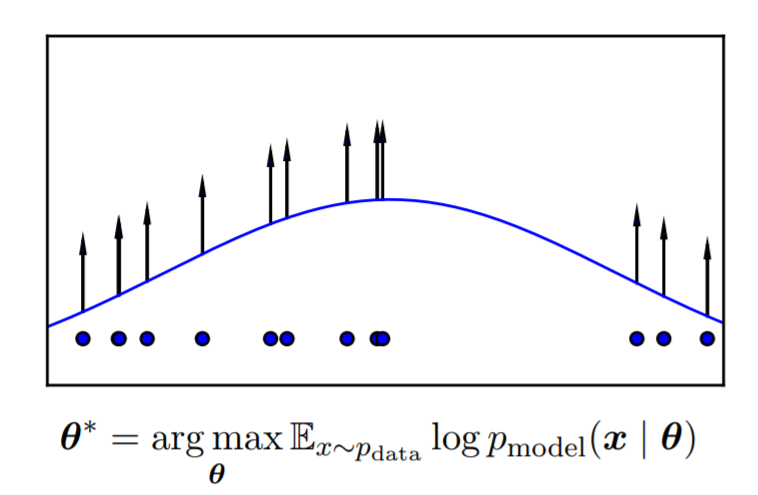
\includegraphics[width=0.45\columnwidth]{master_thesis_template/figs/mll.PNG}
    \caption{An illustration of a ML principle shows how different data points push up different part of the density function. The ML principle takes samples from the training set and then pushes up the probability model assigns to those points. Taken from~\cite{goodfellow2016nips}}
    \label{fig:mll}
\end{figure}

\subsection{Generative Adversarial Networks (GANs)}
\label{subsec:gan}
Learning to sample from high dimensional probability distribution $p_\text{data}$ is complicated and is often an intractable process. However, sampling from simple distribution like Gaussian is well studied and is computationally efficient. 
The key idea behind Generative Adversarial Networks (GANs)~\cite{goodfellow2014generative} is to take samples from simple distribution and apply a non-linear parametric transformation to get samples from high dimensional complex distribution. This learnable transformation is optimized in an adversarial setting.

A GAN consists of two networks namely generator $\mathcal{G}$ and a discriminator $\mathcal{D}$. Consider $p(z)$ to be a prior noise distribution, $\mathcal{X}$ be a set of training samples drawn from data distribution $p_\text{data}$. The network $\mathcal{G}$ transforms samples from noise distribution $z\sim p(z)$ to samples in model distribution $\mathcal{G}(z;\theta_g)$. The network $\mathcal{D}$ takes an input sample $x$ and estimates the probability $\mathcal{D}(x;\theta_d)$ of sample $x$ being drawn from $\mathcal{X}$. Thus a discriminator $\mathcal{D}$ works as a binary classifier with an objective to discriminate between real samples in $\mathcal{X}$ and generated samples $\mathcal{G}(z;\theta_g)$. The objective of generator $\mathcal{G}$ is to generate samples which are similar to real samples and thus can effectively fool the discriminator at the task of classification. 

\subsection{How to train a GAN?}
\label{sub:train_gan}
The objective of generator and discriminator can be interpreted as a minimax game where the generator tries to minimize the gain of the discriminator and the discriminator tries to maximize its gain. Formally, minimax game between $\mathcal{G}$ and $\mathcal{D}$ is expressed by Equation~\ref{eq:gan_loss}. The two players $\mathcal{G}$ and $\mathcal{D}$ are represented by a parametric function and are fully differentiable with respect to their input as well as parameters and thus are typically modeled by neural networks.

\begin{equation}
    \label{eq:gan_loss}
    \min_{\mathcal{G}} \max_{\mathcal{D}} V(\mathcal{D}, \mathcal{G}) = \mathbb{E}_{x\sim p_\text{data}} [\log \mathcal{D}(x)] + \mathbb{E}_{z\sim p(x)} [\log (1 - \mathcal{D}(\mathcal{G}(z))]
\end{equation}

The differentiable nature of $\mathcal{G}$ and $\mathcal{D}$ allows to solve the optimization using gradient based methods. Since the input of one depends on the output of other the optimization is solved in two steps of gradient updates, first updating the parameters of $\theta_g$ and then updating $\theta_d$. Algorithm~\ref{alg:train_sgd_gan} further illustrates the learning of $\mathcal{G}$ and $\mathcal{D}$.

\begin{algorithm}
    \caption{Minibatch stochastic gradient descent training of GAN~\cite{goodfellow2014generative}. For each update of the generator discriminator we update discriminator k number of times, where k is the hyperparameter}
    \label{alg:train_sgd_gan}
    \begin{algorithmic}
        \For{number of iterations}
        \For{k steps}
            \State Sample minibatch of m noise samples from prior $\{z^{(1)},..., z^{(m)}\}\sim p_z(z)$.
            \State Sample minibatch of m samples from data distribution $\{x^{(1)},...,x^{(m)}\} \sim p_\text{data}$.
            \State Update the parameters of discriminator by ascending the stochastic gradient on a minibatch:
            \State $\nabla_{\theta_d} \frac{1}{m} \sum_{i=1}^m [\log \mathcal{D}_{\theta_d}(x^{(i)}) 
             + \log (1 - \mathcal{D}_{\theta_d}(z^{(i)}) )]$
        \EndFor
        \State Sample minibatch of m noise samples from prior $\{z^{(1)},..., z^{(m)}\}\sim p_z(z)$.
        \State Update the generator by descending the stochastic gradient on a minibatch:
        \State $\nabla_{\theta_g} \frac{1}{m}  \sum_{i=1}^m [ \log (1 - \mathcal{D}_{\theta_d}(\mathcal{G}_{\theta_g}(z^{(i)}) )]$
        \EndFor
    \end{algorithmic}
\end{algorithm}

At each step of training, cost of one player depends on the decision of other one. However, both players have no control on the strategy of each other. This results in a zero sum game where loss of one player is equivalent to the benefit of the other one. If both players are optimal then there exist an equilibrium between them referred as Nash Equilibrium. In the NN setting of GAN the optimization problem of both $\mathcal{G}$ and $\mathcal{D}$ is non-convex and the only plausible solution is a local minima which implies an existence of a local Nash equilibrium a state at which cost of $\mathcal{G}$ is minimum w.r.t parameters $\theta_g$ and of $\mathcal{D}$ is minimum w.r.t parameters $\theta_d$~\cite{}.

\subsection{An Information Theoretic Perspective}
In this section we will study the convergence properties of Algorithm~\ref{alg:train_sgd_gan}. Consider $p_\text{data}$ to be the probability distribution of data and $p_\text{g}$ to be the probability distribution learned by the generator $\mathcal{G}$. We want to measure how well probability distribution $p_\text{g}$ approximates distribution $p_\text{data}$. To study the convergence we will consider the $\mathcal{G}$ and $\mathcal{D}$ networks are of infinite capacity. We will first introduce KL Divergence and Jensen Shannon Divergence and will then continue our discussion of optimality.

\subsubsection{Kullback-Leibler Divergence}
\label{subsec:kld}
Kullback-Leibler (KL)
divergence~\cite{kullback1951information} is a measure of discrepancy between two probability distribution. From an information theory point of view a KL-divergence between two probability distribution $P$ and $Q$ is a measure of extra number of bits required to code samples from $P$ when using a code of samples from $Q$. It tells us how much information is lost when $Q$ is used to approximate $P$. Formally, it is defined as:
\begin{equation}
    \label{eq:kld}
    D_{KL} (P || Q) = \mathbb{E}_{x\sim P} \log \frac{P}{Q}
\end{equation}

The KL divergence is a non-negative quantity and is equal to zero if and only if $P=Q$. It is not a proper metric as it is asymmetric and does not obey triangle inequality.

%\begin{equation}
%    \label{eq:kld}
%    D_{KL} (p_\text{data} || p_\text{g}) = \mathbb{E}_{x\sim p_\text{data}} \log \frac{p_\text{data}}{p_\text{g}}
%\end{equation}

\subsubsection{Jensen Shannon Divergence}
\label{subsec:jsd}
Jensen–Shannon divergence is another common measure of similarity between two probability distributions. It is a symmetric and smoothed variant of KL divergence and is defined as:
\begin{equation}
    \label{eq:jen_shan}
    JSD(P,Q) = KL(P||M) + KL(Q||M)
\end{equation}
where $M = \frac{P+Q}{2}$. The choice of $M$ as an average of $P$ and $Q$ further gives an upper bound on divergence. From an information theory sense JSD is regarded as the mutual information between a mixture distribution of $P$ and $Q$ and a random variable indicating the switch between $P$ and $Q$ to produce the mixture.

\subsubsection{Optimality of minimax}
The optimal solution to $V(G,D)$ corresponds to finding a parameter configuration $\theta_g$ that minimizes the objective and $\theta_d$ that maximizes the objective. The optimal discriminator $\mathcal{D}$ for a fixed $\mathcal{G}$ is given by:
\begin{equation}
    \label{eq:opt_gan}
    D_{G}^{\ast}(x) = \frac{p_\text{data}(x)}{p_\text{data}(x) + p_\text{g}(x)}
\end{equation}

For an optimal discriminator the optimization function can be formulated as:
\begin{flalign}
%\begin{aligned}
    C(G) = & \max_D V(G,D) \\
     =&  \mathbb{E}_{x\sim p_\text{data}} [\log \mathcal{D}^\ast(x)] + \mathbb{E}_{z\sim p(z)} [\log (1 - \mathcal{D}^\ast(\mathcal{G}(z))]\\
     =& \mathbb{E}_{x\sim p_\text{data}} [\log \frac{p_\text{data}(x)}{p_\text{data}(x) + p_\text{g}(x)}] + \mathbb{E}_{z\sim p(z)} [\log \frac{p_g(x)}{p_\text{data}(x) + p_\text{g}(x)}]\\
%\end{aligned}
\end{flalign}

For $p_g = p_\text{data}$ the loss function $ C(G)$ can further be expressed as:
\begin{equation}
    C(G) = -\log 4 + 2.JSD(p_\text{data} || p_g)
\end{equation}

As discussed in Section~\ref{subsec:jsd} the $JSD$ is non-negative and takes minimum when two distributions are equal. Thus the optimization problem has a global optimum when $p_g = p_\text{data}$ i.e. with an infinite capacity the generative network can perfectly model the data distribution. Thus in the training process the optimal discriminator aims at estimating the ratio of probability densities as given in Equation~\ref{eq:opt_gan} and the optimal generator aims at minimizing the $JSD$ between $p_g$ and $p_\text{data}$.
%Thus solution is a saddle point where both generator and discriminator are optimal. The optmi


\begin{figure}
    \centering
    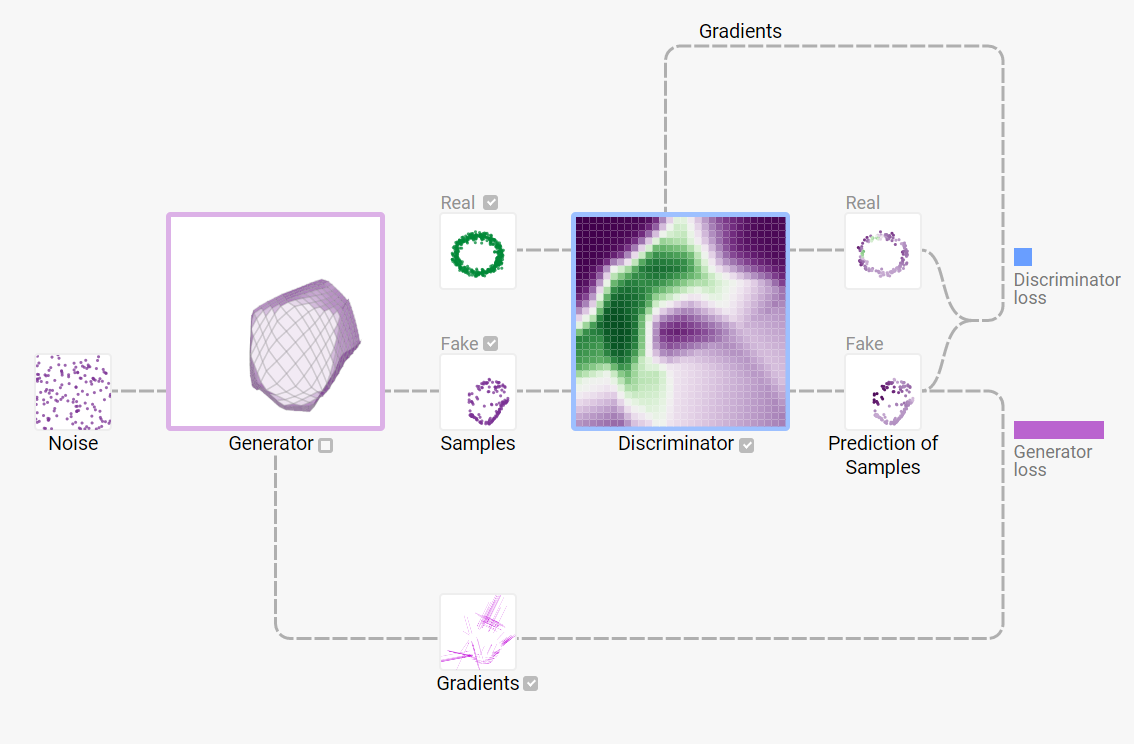
\includegraphics[width=0.75\columnwidth]{master_thesis_template/figs/gan_training.PNG}
    \caption{A geometric illustration of GAN training. Generator learns to transform samples from a simple noise distribution $\mathcal{N}(0,1)$ to complex data distribution. Taken from~\cite{kahng2018gan}}
    \label{fig:gan_train}
\end{figure}
\subsubsection{Challenges in GAN training}
The training of GAN requires finding an equilibrium between generator and discriminator. At each step $\mathcal{G}$ and $\mathcal{D}$ try to undo the progress of each other which makes it difficult to monitor their convergence. Thus the training of GAN is often associated with instability. The two main problem associated with instability are: (i) oscillatory behaviour across modes: this is a situation where generator progressively switches from generating one kind of sample to another without reaching an equilibrium condition. (ii) Mode collapse: in mode collapse generator starts mapping multiple latent noise representation to a single point in data distribution. The more commonly encountered form of model collapse in training of GANs is known as partial mode collapse occurs when generator maps only to a smaller set of training examples resulting in a low diversity of generated samples. This is further explained by asymmetric nature of minimax that is to say:
\begin{equation}
\min_G \max_D V(G,D) \neq \max_G \min_D V(G,D)
\end{equation}
In minimax situation the optimal generator draws sample from data distribution. 
\begin{equation}
    G^\ast = \min_G \max_D V(G,D)
\end{equation}

In case of maxmin the optimal generator lies in the inner loop. As a result it maps every noise distribution to a single data sample. The update methods does not differentiate between minmax and maxmin as a result in some cases the optimization turns out to solve maxmin resulting in the mode collapse. The severity of mode collapse also depends on the diversity of training data. It is more common when training data consists of samples of only few modes. 

Some common metric to look at the diversity of generated samples to understand the situation like mode collapse are inception score~\cite{salimans2016improved}, Fr\'echet inception distance~\cite{heusel2017gans}. We will discuss it in detail in Section~\ref{subsec:eval_metrics}.


\subsection{Variational Auto-encoders}
\label{subsec:vae}
Variational Autoencoder (VAE) introduced by~\cite{kingma2013auto} is an implicit density generative model that learns to encode data. One problem in learning a parametric function to transform simple distribution to complex distribution is that for high dimensional distributions it requires sampling of large number of noise samples $z=\{z_1,...,z_N\}$ to estimate the probability distribution of data $p_\text{data}\approx \frac{1}{N}\sum_i p_g(z_i)$. The large value of $N$ often results in intractability and other training issues. The main idea behind the VAE is to sample $z$ that are more likely to produce samples from $p_\text{data}$. This is achieved by conditioning the distribution of latent $z$ on the training samples $\mathcal{X}$. 

Formally, consider a parametric inference network that outputs statistics of $q(z|X)$, a generator network that outputs a distribution $p_g(X|z)$. A VAE learns to approximate the posteriors $p_g(z|X)$ with $q(z|X)$. This is achieved by optimizing a variational lower bound:
\begin{equation}
    V(x; \theta_1,\theta_2) = - D_{KL}(q_{\theta_1} (z|x)) || p_{\theta_2} (z|x) + \mathbb{E}_{q(z|x)} [\log p_{\theta_2} (x|z)]
\end{equation}

where $\theta_1$ and $\theta_2$ are parameters of inference and generator networks. The gradients of lower bound  with respect to parameters $\theta_1$ are intractable. VAE uses variational calculus to cast the inference as an optimization problem. Consider a given intractable posterior probability distribution $p_{\theta_1}(z|x)$, using variational principle we solve an optimization problem over a family of tractable distributions $\mathcal{F}$. For $q_{\theta_2}(z|x) \in \mathcal{F}$ the optimal approximation is given by:
\begin{equation}
    q\ast = \argmin_{\theta_1} D_{KL} (q_{\theta_1}(z|x) || p_{\theta_2}(z|x))
\end{equation}

We refer to~\cite{doersch2016tutorial} for a more comprehensive discussion of VAE.

\subsection{Cycle GAN}
\label{subsec:cgan}
Cycle GAN~\cite{zhu2017unpaired} is a generative model proposed for unsupervised translation of images between two domains. It is specifically useful for use case like domain adaptation. The key idea behind cycle-GAN is the cycle consistency loss. Consider two set of images of two domains $X=\{x_1,...,x_N\}$ and $Y=\{y_1,...,y_M\}$. The cycle GAN consists of a generator and discriminator for each domain. Let $F$ and $G$ are two generator networks defined as: 
\begin{flalign}
F: X\rightarrow Y\\
G: Y\rightarrow X
\end{flalign}
Let $D_{X}$ and $D_{Y}$ be two discriminator networks defined as:
\begin{flalign}
D_X: X\rightarrow \mathcal{R}\\
D_Y: Y\rightarrow \mathcal{R}
\end{flalign}
Discriminator $D_X$ is trained to discriminate between original images in $X$ and generated images $G(X)$ likewise $D_Y$ is trained to discriminate between original images in $Y$ and generated images $F(Y)$. The combined training loss of two GANs is expressed as:
\begin{flalign}
V_\text{GAN} (F,D_Y,G,D_X) = V_\text{GAN} (F,D_Y,X,Y) +  V_\text{GAN} (G,D_X,X,Y)
\end{flalign}
One essential constraint imposed in cycle GAN is of cycle consistency loss. It is to make sure when an image is translated from one domain to another it should preserve certain attributes of original domain. This is done by constraining $F$ and $G$ to be inverse mapping of each other. Specifically:
\begin{flalign}
F \circ G = I_{Y}\\     
G \circ F = I_{X}
\end{flalign}
The cyclic loss term is defined is as:
\begin{equation}
    V_\text{cyc}(F,D_Y,G,D_X) = ||X-G(F(X)||_1 + ||Y-F(G(X)||_1  
\end{equation}
The full optimization term is expressed as:
\begin{equation}
    F^\ast, G^\ast = \argmin_{F,G}\max_{D_X,D_Y} V_\text{GAN}(F,G,D_X,D_Y) +   V_\text{cyc}(F,D_Y,G,D_X) 
\end{equation}

Figure~\ref{fig:cycle_gan} gives a geometric view of cycleGAN. The cycle consistency loss prevents problem of mode collapse by forcing network to retain certain features of original domain.

\begin{figure}
    \centering
    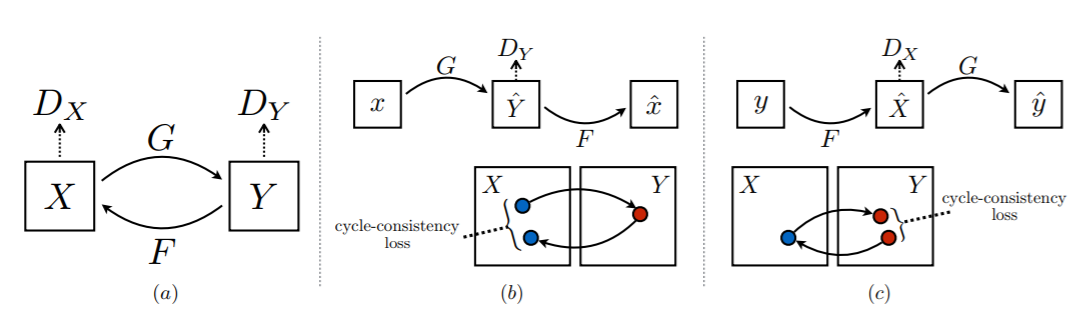
\includegraphics[width=0.95\columnwidth]{master_thesis_template/figs/cycle_gan.PNG}
    \caption{An illustration of mapping in cycle-GAN. (a) The model contains a pair of generator discriminator networks $(F, D_Y)$ and $(G,D_X)$ where $F: X\rightarrow Y$ and $G: Y\rightarrow X$ are generator networks and $D_Y: Y\rightarrow \mathcal{R}$ and $D_X: X\rightarrow \mathcal{R}$ are corresponding discriminator networks, (b) and (c) demonstrate cycle consistency for two domains. Taken from~\cite{zhu2017unpaired}}
    \label{fig:cycle_gan}
\end{figure}



\subsection{UNIT:VAE-Coupled-GAN}
\label{subsec:unit_gan}
Unsupervised image to image translation (UNIT) is another GAN based framework for unpaired translation of images between two domain. In this thesis, our work is inspired by the UNIT framework. The UNIT~\cite{liu2017unsupervised} is based on the assumption that two domain $X$ and $Y$ have an underlying joint probability distribution $P_{X,Y}(x,y)$ and the objective is to approximate $P_{X,Y}(x,y)$ from two marginal distribution $P_{X}(x)$ and $P_{Y}(y)$. Inferring a joint distribution from marginal distribution is an ill-posed problem. The UNIT approximates joint probability distribution under an assumption that two domain have a shared latent space $\mathcal{Z}$. 


Unlike cycle-GAN in UNIT the two generator are expressed as a pair of encoder-decoder $(E_1,G_1)$ for domain $X$ and $(E_2,G_2)$ for domain $Y$ and the corresponding discriminators $D_1$ and $D_2$. For any pair of images $(x,y)$ where $x\in X$ and $y\in Y$ there exist a representation in shared latent space $z\in\mathcal{Z}$ as:
\begin{equation}
    z = E_1(x) = E_2(y)
\end{equation}

and the mapping from $z\in\mathcal{Z}$ to image space is given by:
\begin{flalign}
    x = G_1(z)\\
    y=G_2(z)
\end{flalign}

The concept of shared latent space is implemented by imposing following two conditions: (i) Weight sharing of last layer of encoder network and first layer of decoder network. (ii) cycle consistency loss. The (i) is a more strict condition it also implies cycle consistency, (ii) is imposed as a constraint to restrict the search space of network and avoid problems like mode collapse. Figure~\ref{fig:vae-gan}
gives a geometric view of shared latent space and UNIT network.

The VAE-GAN loss of two generators is defined as:
\begin{equation}
\begin{aligned}
V_\text{VAE-GAN} (E_1,G_1,E_2,G_2,D_1,D_2) = & V_\text{VAE} (E_1,G_1,X,Y) +  V_\text{GAN} (E_2,G_1,D_1,X,Y) \\ 
&+ V_\text{VAE} (E_2,G_2,X,Y) +  V_\text{GAN} (E_1,G_2,D_2,X,Y)
\end{aligned}
\end{equation}

The cycle consistency loss is expressed like a VAE objective function given by:
\begin{equation}
\begin{aligned}
     V_{\text{cyc}_1}(E_1,G_1,E_2,G_2) =& \lambda_1 D_{KL} (q_1(z_x|x_X) || p_Z(z)) + \lambda_2 D_{KL} (q_2(z_y|x_X^{X2Y}) || p_Z(z))\\
    & + \lambda_3 \mathbb{E}_{z_y\sim q_2(z_y|x_X^{X2Y}}) [\log p_{G_1}(x_X|z_y)]       
\end{aligned}
\end{equation}

\begin{equation}
\begin{aligned}
    V_{\text{cyc}_2}(E_2,G_2,E_1,G_1) =& \lambda_1 D_{KL} (q_2(z_2|y_Y) || p_Z(z)) + \lambda_2 D_{KL} (q_1(z_x|y_Y^{Y2X}) || p_Z(z))\\
    & + \lambda_3 \mathbb{E}_{z_x\sim q_1(z_x|y_Y^{Y2X}}) [\log p_{G_1}(x_X|z_x)]
\end{aligned}
\end{equation}

\begin{equation}
 V_{\text{cyc}}(E_1,G_1,E_2,G_2)  = V_{\text{cyc}_1}(E_1,G_1,E_2,G_2) + V_{\text{cyc}_2}(E_2,G_2,E_1,G_1)
\end{equation}
    
where $p_Z(z)=\mathcal{N}(z|0,I)$ is a prior distribution assumed to be Gaussian. The KL term ensures latent space distribution is close to prior and the negative log-likelihood term is similar to consistency term in cycleGAN and ensures $G_1(E_2(G_2(E_1(X)))\sim X$ and $G_1(E_2(G_2(E_1(Y)))\sim Y$. 

The full optimization problem of UNIT is expressed as:
\begin{equation}
    \begin{aligned}
        E_1^\ast, E_2^\ast, G_1^\ast, G_2^\ast, D_1^\ast, D_2^\ast =& \argmin_{E_1,G_1,E_2,G_2} \max_{D_1, D_2} V_\text{VAE-GAN} (E_1,G_1,E_2,G_2,D_1,D_2)\\
        &\qquad \qquad \qquad +  V_\text{cyc}(E_1,G_1,E_2,G_2)
    \end{aligned}
\end{equation}

\begin{figure}
    \centering
    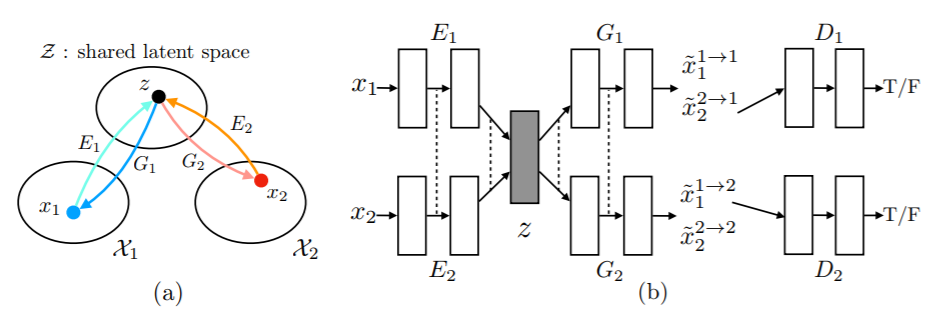
\includegraphics[width=0.95\columnwidth]{master_thesis_template/figs/unit.PNG}
    \caption{UNIT Network:  $(E_1,G_1)$ and $(E_2,G_2)$ are two pairs of VAE and $D_1$ and $D_2$ are two discriminators corresponding to domain $X$ and $Y$. (a) An Illustration of shared latent space $\mathcal{Z}$. The UNIT assumes pair $(x_1,x_2)$ can be represented by a shared latent embedding $z\in\mathcal{Z}$. (b) An example of UNIT network where dotted line illustrates weight sharing. Taken from~\cite{liu2017unsupervised}}
    \label{fig:vae-gan}
\end{figure}



\section{Deep Generative Models for Audio Signals}
\label{subsec:dganaudio}
In this section we review recent work on deep generative models for audio signals. The recent development in generative models in particular GANs have already achieved lot of success for image data. However, the application to audio signals is still in the early stage. The WaveNet~\cite{oord2016wavenet} proposed an autoregressive generative model for high quality audio synthesis. One key drawback with this approach is it works in time domain and its autoregressive nature results in slow inference for audio data sampled at high frequency. 

One alternative to this approach is to use compressed $STFT$ representation instead of time domain representation of a signal. In our previous discussion we looked at the problem of consistency and phase reconstruction associated with this approach. A recent work of ~\cite{engel2019gansynth} address this problem by learning a generative model for full spectrogram representation. To deal with the hardness of phase spectra authors use an alternative representation of phase namely instantaneous frequency (IF). In ~\cite{marafiotiadversarial} authors proposed a GAN network with an additional constraint to learn consistent spectrogram representation. The consistency condition further speed up the learning of an iterative algorithm for phase reconstruction and provides better quality audio synthesis.

Domain adaptation of audio signals in particular speech data offers a promising direction to improve ASR systems, development of robust speaker detection system, privacy in end to end dialogue systems and many more exciting problems. In~\cite{hosseini2018multi} introduced a cycleGAN based network using spectrogram representation for cross domain adaptation of speech signals. The approach makes use of multiple discriminator based on frequency band to allow generator to focus on fine grained features.

In~\cite{kaneko2017parallel} proposed an architecture utilizing an idea of cycleGAN for converting voice of one speaker to another. The approach is evaluated on VCC 2016 dataset~\cite{nakashika2016non} of 10 speakers. In~\cite{huang2018voice} proposed VAE based architecture for voice conversion. The network jointly uses two types of spectral features in VAE setting.
In a very recent work~\cite{qian2019autovc} proposed an autoencoder framework for zero shot voice conversion. The conversion is done by incorporating speaker encoding obtained from a separate pre-trained network. The pretrained network is trained on the task of speaker detection on a large corpus of $3549$ speakers. The decoder of an autoencoder network is conditioned on this embedding.

